% (find-LATEX "2021-1-C3-notacao-de-fisicos.tex")
% (defun c () (interactive) (find-LATEXsh "lualatex -record 2021-1-C3-notacao-de-fisicos.tex" :end))
% (defun C () (interactive) (find-LATEXsh "lualatex 2021-1-C3-notacao-de-fisicos.tex" "Success!!!"))
% (defun D () (interactive) (find-pdf-page      "~/LATEX/2021-1-C3-notacao-de-fisicos.pdf"))
% (defun d () (interactive) (find-pdftools-page "~/LATEX/2021-1-C3-notacao-de-fisicos.pdf"))
% (defun e () (interactive) (find-LATEX "2021-1-C3-notacao-de-fisicos.tex"))
% (defun l () (interactive) (find-LATEX "2021-1-C3-3D.lua"))
% (defun o () (interactive) (find-LATEX "2020-2-C3-plano-tang.tex"))
% (defun u () (interactive) (find-latex-upload-links "2021-1-C3-notacao-de-fisicos"))
% (defun v () (interactive) (find-2a '(e) '(d)))
% (defun d0 () (interactive) (find-ebuffer "2021-1-C3-notacao-de-fisicos.pdf"))
% (defun cv () (interactive) (C) (ee-kill-this-buffer) (v) (g))
%          (code-eec-LATEX "2021-1-C3-notacao-de-fisicos")
% (find-pdf-page   "~/LATEX/2021-1-C3-notacao-de-fisicos.pdf")
% (find-sh0 "cp -v  ~/LATEX/2021-1-C3-notacao-de-fisicos.pdf /tmp/")
% (find-sh0 "cp -v  ~/LATEX/2021-1-C3-notacao-de-fisicos.pdf /tmp/pen/")
%     (find-xournalpp "/tmp/2021-1-C3-notacao-de-fisicos.pdf")
%   file:///home/edrx/LATEX/2021-1-C3-notacao-de-fisicos.pdf
%               file:///tmp/2021-1-C3-notacao-de-fisicos.pdf
%           file:///tmp/pen/2021-1-C3-notacao-de-fisicos.pdf
% http://angg.twu.net/LATEX/2021-1-C3-notacao-de-fisicos.pdf
% (find-sh0 "cp -v ~/usrc/silvanus/33283-t.pdf /tmp/silvanus.pdf")
%                             (find-xournalpp "/tmp/silvanus.pdf")
% (find-LATEX "2019.mk")
% (find-CN-aula-links "2021-1-C3-notacao-de-fisicos" "3" "c3m211nf" "c3nf")

% «.video-1»			(to "video-1")
% «.video-2»			(to "video-2")
% «.video-3»			(to "video-3")
% «.video-4»			(to "video-4")
%
% «.defs»			(to "defs")
% «.title»			(to "title")
% «.introducao»			(to "introducao")
% «.links»			(to "links")
% «.silvanus-thompson»		(to "silvanus-thompson")
% «.primeiro-exemplo»		(to "primeiro-exemplo")
% «.omitir-nomes»		(to "omitir-nomes")
% «.omitir-nomes-2»		(to "omitir-nomes-2")
% «.exercicio-1»		(to "exercicio-1")
% «.exercicio-2»		(to "exercicio-2")
% «.silvanus-triangle»		(to "silvanus-triangle")
% «.quadraticas-exemplos»	(to "quadraticas-exemplos")
% «.thomas»			(to "thomas")
% «.bortolossi»			(to "bortolossi")
% «.segundo-exemplo»		(to "segundo-exemplo")
%
% «.djvuize»			(to "djvuize")


% «video-1»  (to ".video-1")
% (find-ssr-links "c3m211nf" "2021-1-C3-notacao-de-fisicos" "fMNgr5wDMek")
% (code-video     "c3m211nfvideo" "$S/http/angg.twu.net/eev-videos/2021-1-C3-notacao-de-fisicos.mp4")
% (find-c3m211nfvideo "0:00")
% (find-c3m211nfvideo "0:10" "ainda como entender visualmente derivadas parciais")
% (find-c3m211nfvideo "0:42" "derivadas parciais")
% (find-c3m211nfvideo "0:57" "derivadas totais")
% (find-c3m211nfvideo "1:20" "lembrem do truque")
% (find-c3m211nfvideo "1:35" "que as variáveis variam juntas")
% (find-c3m211nfvideo "2:15" "nomes que deixem claro de que xzes eles vêm")
% (find-c3m211nfvideo "2:55" "derivada como limite")
% (find-c3m211nfvideo "3:42" "várias notações: quando a gente define")
% (find-c3m211nfvideo "4:23" "pra calcular a derivada num determinado x")
% (find-c3m211nfvideo "4:34" "primeiro o caso geral")
% (find-c3m211nfvideo "4:58" "e depois especializa")
% (find-c3m211nfvideo "5:12" "exatamente a mesma coisa com as derivadas parciais")
% (find-c3m211nfvideo "5:20" "z = F(x,y)")
% (find-c3m211nfvideo "5:55" "o que vai fazer esses truques ficarem claros")
% (find-c3m211nfvideo "6:02" "que a gente só pode usar como abreviação")
% (find-c3m211nfvideo "6:13" "1o caso que nos interessa")
% (find-c3m211nfvideo "6:32" "y = f(x), z = g(y)")
% (find-c3m211nfvideo "6:45" "como é que a gente visualiza isso")
% (find-c3m211nfvideo "6:55" "à medida que o x varia")
% (find-c3m211nfvideo "7:35" "podemos pensar como sendo uma tabela")
% (find-c3m211nfvideo "7:52" "y = x + 4, z = 10x")
% (find-c3m211nfvideo "8:15" "caso geral")
% (find-c3m211nfvideo "8:25" "z = g(f(x))")
% (find-c3m211nfvideo "9:12" "o que acontece quando o x varia")
% (find-c3m211nfvideo "9:43" "Δz/Δx")
% (find-c3m211nfvideo "10:05" "primeira variável e segunda variável")
% (find-c3m211nfvideo "10:20" "derivada na segunda variável")
% (find-c3m211nfvideo "10:28" "uma notação parecida mesmo nesse caso simples")
% (find-c3m211nfvideo "10:42" "y_x =")
% (find-c3m211nfvideo "10:48" "z_y =")
% (find-c3m211nfvideo "11:05" "d/dx f(x) =")
% (find-c3m211nfvideo "11:20" "g'(y)")
% (find-c3m211nfvideo "11:30" "z_x = ?")
% (find-c3m211nfvideo "11:43" "d ao invés de Δ")
% (find-c3m211nfvideo "11:56" "dz/dy dy/dx")
% (find-c3m211nfvideo "12:00" "cancelam")
% (find-c3m211nfvideo "12:15" "notação curtíssima")
% (find-c3m211nfvideo "12:28" "ponto base")
% (find-c3m211nfvideo "12:45" "a expansão vai ser a seguinte")
% (find-c3m211nfvideo "13:12" "só que y é f(x)")
% (find-c3m211nfvideo "13:56" "quando a gente for olhar derivadas parciais")
% (find-c3m211nfvideo "14:18" "z = F(x,y)")
% (find-c3m211nfvideo "14:48" "a gente geralmente não vai escrever")
% (find-c3m211nfvideo "14:54" "default: ponto base")
% (find-c3m211nfvideo "15:08" "se a gente não escrever o argumento")
% (find-c3m211nfvideo "15:45" "z = F(x,y) nos dá uma superfície")
% (find-c3m211nfvideo "16:10" "digamos que a gente tem uma trajetória aqui")
% (find-c3m211nfvideo "16:40" "à medida que o t varia")
% (find-c3m211nfvideo "16:55" "o que acontece quando a gente varia o t um pouquinho?")
% (find-c3m211nfvideo "17:15" "anda pra um outro ponto pertinho")
% (find-c3m211nfvideo "18:20" "quando Δt for muito pequeno")
% (find-c3m211nfvideo "18:48" "onde isso aqui é uma derivada parcial")
% (find-c3m211nfvideo "19:20" "confuso mas dá pra trabalhar nas duas linguagens ao mesmo tempo")
% (find-c3m211nfvideo "20:18" "a gente vai aprender a fazer a tradução")
% (find-c3m211nfvideo "20:50" "terceiro exemplo")

% «video-2»  (to ".video-2")
% (find-ssr-links "c3m211nf2" "2021-1-C3-notacao-de-fisicos-2" "bjBlOqO-7Do")
% (code-video "c3m211nf2video" "$S/http/angg.twu.net/eev-videos/2021-1-C3-notacao-de-fisicos-2.mp4")
% (find-c3m211nf2video "0:00")

% «video-3»  (to ".video-3")
% (find-ssr-links "c3m211nfstr" "2021-1-C3-notacao-de-fisicos-s-tr" "{aindanaosubiproyt}")
% (code-video "c3m211nfstrvideo" "$S/http/angg.twu.net/eev-videos/2021-1-C3-notacao-de-fisicos-s-tr.mp4")
% (find-c3m211nfstrvideo "0:00")

% «video-4»  (to ".video-4")
% (find-ssr-links "c3m211nfsesc" "2021-1-C3-notacao-de-fisicos-s-esc" "{aindanaosubiproyt}")


\documentclass[oneside,12pt]{article}
\usepackage[colorlinks,citecolor=DarkRed,urlcolor=DarkRed]{hyperref} % (find-es "tex" "hyperref")
\usepackage{amsmath}
\usepackage{amsfonts}
\usepackage{amssymb}
\usepackage{pict2e}
\usepackage[x11names,svgnames]{xcolor} % (find-es "tex" "xcolor")
\usepackage{colorweb}                  % (find-es "tex" "colorweb")
%\usepackage{tikz}
%
% (find-dn6 "preamble6.lua" "preamble0")
%\usepackage{proof}   % For derivation trees ("%:" lines)
%\input diagxy        % For 2D diagrams ("%D" lines)
%\xyoption{curve}     % For the ".curve=" feature in 2D diagrams
%
\usepackage{edrx21}               % (find-LATEX "edrx21.sty")
\input edrxaccents.tex            % (find-LATEX "edrxaccents.tex")
\input edrx21chars.tex            % (find-LATEX "edrx21chars.tex")
\input edrxheadfoot.tex           % (find-LATEX "edrxheadfoot.tex")
\input edrxgac2.tex               % (find-LATEX "edrxgac2.tex")
%
%\usepackage[backend=biber,
%   style=alphabetic]{biblatex}            % (find-es "tex" "biber")
%\addbibresource{catsem-slides.bib}        % (find-LATEX "catsem-slides.bib")
%
% (find-es "tex" "geometry")
\usepackage[a6paper, landscape,
            top=1.5cm, bottom=.25cm, left=1cm, right=1cm, includefoot
           ]{geometry}
%
\begin{document}

\catcode`\^^J=10
\directlua{dofile "dednat6load.lua"}  % (find-LATEX "dednat6load.lua")

%L dofile "edrxtikz.lua"     -- (find-LATEX "edrxtikz.lua")
%L dofile "edrxpict.lua"     -- (find-LATEX "edrxpict.lua")
%L dofile "2021-1-C3-3D.lua" -- (find-LATEX "2021-1-C3-3D.lua")
%L
%L V3.__index.tostring = function (v) return v:v2string() end
\pu

\pu

% «defs»  (to ".defs")
% (find-LATEX "edrx15.sty" "colors-2019")
\long\def\ColorRed   #1{{\color{Red1}#1}}
\long\def\ColorViolet#1{{\color{MagentaVioletLight}#1}}
\long\def\ColorViolet#1{{\color{Violet!50!black}#1}}
\long\def\ColorGreen #1{{\color{SpringDarkHard}#1}}
\long\def\ColorGreen #1{{\color{SpringGreenDark}#1}}
\long\def\ColorGreen #1{{\color{SpringGreen4}#1}}
\long\def\ColorGray  #1{{\color{GrayLight}#1}}
\long\def\ColorGray  #1{{\color{black!30!white}#1}}
\long\def\ColorBrown #1{{\color{Brown}#1}}
\long\def\ColorBrown #1{{\color{brown}#1}}
\long\def\ColorOrange#1{{\color{orange}#1}}

\long\def\ColorShort #1{{\color{SpringGreen4}#1}}
\long\def\ColorLong  #1{{\color{Red1}#1}}

\def\pictgray#1{{\color{GrayPale}\linethickness{0.3pt}#1}}

\def\frown{\ensuremath{{=}{(}}}
\def\True {\mathbf{V}}
\def\False{\mathbf{F}}
\def\D    {\displaystyle}

\def\drafturl{http://angg.twu.net/LATEX/2021-1-C3.pdf}
\def\drafturl{http://angg.twu.net/2021.1-C3.html}
\def\draftfooter{\tiny \href{\drafturl}{\jobname{}} \ColorBrown{\shorttoday{} \hours}}



%  _____ _ _   _                               
% |_   _(_) |_| | ___   _ __   __ _  __ _  ___ 
%   | | | | __| |/ _ \ | '_ \ / _` |/ _` |/ _ \
%   | | | | |_| |  __/ | |_) | (_| | (_| |  __/
%   |_| |_|\__|_|\___| | .__/ \__,_|\__, |\___|
%                      |_|          |___/      
%
% «title»  (to ".title")
% (c3m211nfp 1 "title")
% (c3m211nfa   "title")

\thispagestyle{empty}

\begin{center}

\vspace*{1.2cm}

{\bf \Large Cálculo 3 - 2021.1}

\bsk

Aula 14: Notação de físicos

\bsk

Eduardo Ochs - RCN/PURO/UFF

\url{http://angg.twu.net/2021.1-C3.html}

\end{center}

\newpage

% «introducao»  (to ".introducao")
% (c3m211nfp 2 "introducao")
% (c3m211nfa   "introducao")

{\bf Introdução}

% (find-bortolossi5page (+ -162 164) "5.2. Definições e exemplos")
% (find-bortolossi5page (+ -162 165)   "Fig. 5.2: Interpretação geométrica")
% (find-bortolossi5page (+ -162 167)   "Exemplo 5.1: Cobb-Douglas")
% (find-bortolossi5page (+ -162 170)   "derivada parcial")
% (find-bortolossi5page (+ -162 171)   "a notação D_1 f é a mais clara")
% (find-bortolossi5page (+ -162 172)   "omitir os pontos onde as parciais são calculadas")

Na página 170--172 do cap.5 o Bortolossi fala de algumas convenções
sobre variáveis que ele vai usar o mínimo possível, porque elas às
vezes são difíceis de interpretar e às vezes são ambíguas...

Isso é um assunto bem maior e mais complicado do que parece. Quando eu
fiz graduação em algumas matérias essas convenções -- que eu vou
chamar de ``notação de físicos'' -- eram totalmente
\ColorRed{proibidas}, mas em outras elas eram tratadas como algo
\ColorRed{óbvio} que \ColorRed{todo mundo sabia usar}.

A gente vai aprender alguns dos princípios por trás da ``notação de
físicos'' e vamos como usar essa ``notação de físicos'' como uma
\ColorRed{abreviação} pra uma notação muito menos ambígua que
matemáticos ``estritos'' aceitam.


\newpage

% «links»  (to ".links")
% (c3m211nfp 3 "links")
% (c3m211nfa   "links")

{\bf Links (pra matemáticos que estiverem lendo isso aqui)}

%\msk

Eu aprendi ``notação de físicos'' estudando EDPs pelo livro do

Fritz John e estudando Cálculo de Variações:

%\ssk

{\footnotesize

\url{https://www.springer.com/gp/book/9781461599661} Fritz John

% \url{https://math.stackexchange.com/questions/44828/introductory-text-for-calculus-of-variations}

% \url{https://mathoverflow.net/questions/129122/good-book-on-calculus-of-variations}

\url{http://www-users.math.umn.edu/~olver/ln_/cv.pdf} Olver

}

%\ssk

e um pouco pelos livros do Física do Moysés Nussenzveig.

\bsk

O ``The Language of Mathematics'' do Mohan Ganesalingam 

em coisas muito boas sobre variáveis.
\href{https://www.amazon.com/Language-Mathematics-Linguistic-Philosophical-Investigation/dp/364237011X}{Amazon},
\href{https://www.maa.org/press/maa-reviews/the-language-of-mathematics}{MAA
  Reviews}.


\bsk

Andrej Bauer: ``\href{http://math.andrej.com/2021/06/24/the-dawn-of-formalized-mathematics/}{The
  dawn of formalized mathematics}''.

% http://math.andrej.com/asset/data/the-dawn-of-formalized-mathematics.pdf#page=15
A partir do
\href{http://math.andrej.com/asset/data/the-dawn-of-formalized-mathematics.pdf\#page=15}{slide
  15}.



\newpage

{\bf Mais links (pra matemáticos)}

\bsk

{\footnotesize

\url{https://en.wikipedia.org/wiki/Physical_quantity}

\url{https://en.wikipedia.org/wiki/Dependent_and_independent_variables}

\url{https://en.wikipedia.org/wiki/Variable_(mathematics)}

\url{https://en.wikipedia.org/wiki/Variable_(computer_science)}

\msk

% (find-books "__analysis/__analysis.el" "redish-gupta")
%
Redish/Gupta: ``\href{https://arxiv.org/pdf/1002.0472.pdf}{Making
  Meaning with Math in Physics: A Semantic Analysis}''

\msk

Ellermeijer/Heck: ``Differences between the use of mathematical entities

in mathematics and physics and the consequences for an integrated learning

environment.''
\href{https://staff.fnwi.uva.nl/a.j.p.heck/research/art/girep2001.pdf\#page=6}{Page
  6}.

}



\newpage

% «silvanus-thompson»  (to ".silvanus-thompson")
% (c3m211nfp 3 "silvanus-thompson")
% (c3m211nfa   "silvanus-thompson")
% (find-books "__analysis/__analysis.el" "thompson")

{\bf Silvanus P.~Thompson: Calculus Made Easy (1910)}

Vou usar bastante o livro do Silvanus P.~Thompson...

Ele está em inglês, mas descobri uma versão em \LaTeX{} dele 

feita a partir de uma versão em domínio público --- esta aqui:

\ssk

{\footnotesize

\url{https://www.gutenberg.org/files/33283/33283-pdf.pdf}

}

\ssk

que eu consigo modificar. Vou tentar traduzir algumas

páginas dessa versão pra português.

\msk

Links pra uma versão em HTML do livro

e pra comentários sobre ela:

\ssk

{\footnotesize

\url{https://calculusmadeeasy.org/}

\url{https://avidemia.com/calculus-made-easy/}

\url{https://news.ycombinator.com/item?id=27991120}

\url{https://news.ycombinator.com/from?site=calculusmadeeasy.org}

}

\bsk

\standout{Obs:} o Silvanus não distingue $dx$ de $Δx$.





\newpage

% «primeiro-exemplo»  (to ".primeiro-exemplo")
% (c3m211nfp 5 "primeiro-exemplo")
% (c3m211nfa   "primeiro-exemplo")

{\bf Um primeiro exemplo}

Digamos que $y=\sqrt{x}$.

Podemos considerar que $x$ e $y$ ``variam juntos'',

``obedecendo certas restrições''. O conjunto dos pontos $(x,y)$

que obedecem essas restrições é $\setofxyst{y = \sqrt{x}}$,

e o gráfico é:
%
% (find-latexscan-links "C3" "20210804_sqrt")
% (find-xpdf-page "~/LATEX/2021-1-C3/20210804_sqrt.pdf")
$$\myvcenter{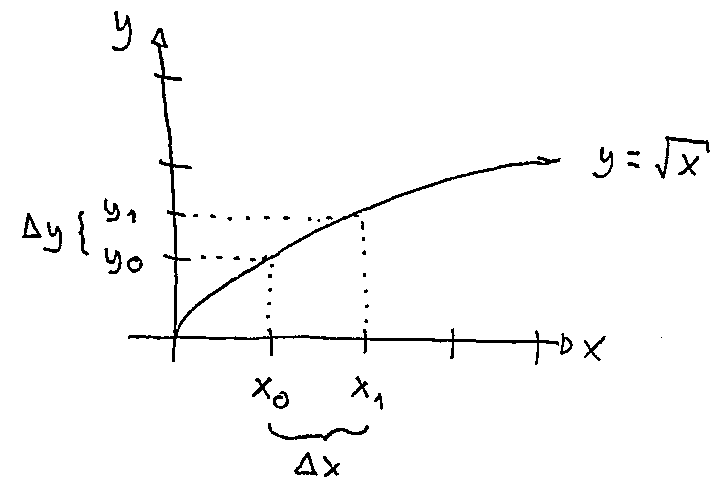
\includegraphics[height=4cm]{2021-1-C3/20210804_sqrt.pdf}}$$

\newpage

{\bf Um primeiro exemplo (2)}

Em geral vamos considerar que $x_0$ é ``mais fixo'' do que $x_1$.

Quando dizemos ``diminua $Δx$; ele era 1 e passa a ser 0.5''

o $x_0$ não muda e o $x_1$ sim --- e temos $y_0 = \sqrt{x_0}$, $y_1 = \sqrt{x_1}$,

$Δy = y_1-y_0$.

\msk

O Silvanus Thompson usa os termos ``independent variable''

e ``dependent variable''. Neste exemplo nós vamos considerar

que $x_0$ e $x_1$ são as variáveis independentes, e que a partir

dos valores delas dá pra calcular os valores das variáveis

dependentes, que são $Δx$, $y_0$, $y_1$, e $Δy$.

% (find-sthompsonpage (+ 11  14)   "dependent variable")
% (find-sthompsontext (+ 11  14)   "dependent variable")

\msk

Também daria pra considerar que as variáveis independentes

são $x_0$ e $Δx$... aí $x_1$ passaria a ser uma das variáveis

dependentes.


\newpage

% «omitir-nomes»  (to ".omitir-nomes")
% (c3m211nfp 8 "omitir-nomes")
% (c3m211nfa   "omitir-nomes")

{\bf O truque de omitir nomes de funções}

\ssk

O ``normal'' seria a gente dizer que $y = f(x) = \sqrt{x}$,

mas os ``físicos'' às vezes dizem só:
%
$$y = y(x) = \sqrt{x}$$

e aí em contextos em que a letra $y$ é usada como

um nome de função ela é interpretada como $f$...

Aí a gente vai ter coisas como:
%
\def\limdx{\lim_{Δx→0}}
%
$$\frac{dy}{dx} = \limdx \frac{Δy}{Δx} = f'(x_0)$$

Veja as contas do próximo slide.

\newpage

% «omitir-nomes-2»  (to ".omitir-nomes-2")
% (c3m211nfp 9 "omitir-nomes-2")
% (c3m211nfa   "omitir-nomes-2")

{\bf O truque de omitir nomes de funções (2)}

\ssk

$$\begin{array}{rcl}
  \D \frac{dy}{dx} &=& \D \limdx \frac{Δy}{Δx}        \\[10pt]
                   &=& \D \limdx \frac{y_1 - y_0}{Δx} \\[10pt]
                   &=& \D \limdx \frac{y(x_1) - y(x_0)}{Δx} \\[10pt]
                   &=& \D \limdx \frac{y(x_0 + Δx) - y(x_0)}{Δx} \\[10pt]
                   &=& \D \limdx \frac{f(x_0 + Δx) - f(x_0)}{Δx} \\[10pt]
                   &=& f'(x_0) \\
  \end{array}
$$

\newpage

% «exercicio-1»  (to ".exercicio-1")
% (c3m211nfp 10 "exercicio-1")
% (c3m211nfa    "exercicio-1")

{\bf Exercício 1}

\ssk

Assista este vídeo do 6:13 até o 12:56:

\ssk

{\footnotesize

\url{http://angg.twu.net/eev-videos/2021-1-C3-notacao-de-fisicos.mp4}

\url{https://www.youtube.com/watch?v=fMNgr5wDMek}

}

\ssk

Ele explica como a regra da cadeia vira algo super curto

na ``notação de físicos''.

\msk

a) Calcule $z_{xx}$ usando a ``notação de físicos''.

b) Traduza as suas contas pra notação convencional.

\msk

No item a você encontrou uma fórmula geral.

Agora vamos aplicá-las em casos específicos pra testá-la.

\msk

c) Especialize as suas contas do item a pro caso

\phantom{c) }$z(y) = \sen y$, $y(x) = e^{4x}$.

d) Calcule $\frac{d}{dx}\frac{d}{dx} \sen(e^{4x})$ pelo método convencional.


\newpage

{\bf Derivadas parciais e derivadas totais}

Digamos que $z = z(x,y)$ e $y = y(x)$.

\msk

Vamos começar com um caso bem concreto --- um que

eu usei em EDOs com variáveis separáveis em C2... link:
\ssk

{\footnotesize

\url{http://angg.twu.net/LATEX/2020-2-C2-edovs.pdf}

}

\msk

O nosso caso bem concreto vai ser:

$z = z(x,y) = x^2 + y^2$,

$y = y(x) = \sqrt{1 - x^2}$.

quando nós \ColorRed{só} consideramos o $z = z(x,y) = x^2 + y^2$

as derivadas parciais de $z$ são $z_x = 2x$ e $z_y = 2y$,

mas quando \ColorRed{também} consideramos o $y = y(x) = \sqrt{1 - x^2}$

aí temos $z = z(x,y(x)) = x^2 + \sqrt{1-x^2}^2 = 1$, e $\frac{dz}{dx}=0$.

\msk

Esta derivada $\frac{dz}{dx} = \frac{d}{dx} z(x,y(x))$ é chamada de

\ColorRed{derivada total} de $z$ com relação a $y$.




\newpage

% «exercicio-2»  (to ".exercicio-2")
% (c3m211nfp 12 "exercicio-2")
% (c3m211nfa    "exercicio-2")

{\bf Exercício 2.}

Digamos que $z = z(x,y) = (x+2)(y+3)$

e que $y = y(x) = \sen x$.

a) Calcule $\frac{∂z}{∂x}$, $\frac{∂z}{∂y}$.

b) Calcule $\frac{dz}{dx}$.

c) Calcule $\frac{d}{dx}\frac{d}{dx}z$.

\msk

\ColorRed{Convenção:} quando uma expressão como $z_x$ puder

ser interpretada tanto como uma derivada parcial quanto

como uma derivada total o default é interpretá-la

como derivada parcial.


\newpage

{\bf Exercício 3.}

Digamos que $z=z(x,y)$ e $y=y(x)$.

(Isto é uma versão mais geral do exercício 2).

\ssk

a) Calcule $\frac{d}{dx}z$.

\ssk

b) Calcule $\frac{d}{dx}\frac{d}{dx}z$.




\newpage

% «silvanus-triangle»  (to ".silvanus-triangle")
% (c3m211nfp 14 "silvanus-triangle")
% (c3m211nfa    "silvanus-triangle")
% (find-books "__analysis/__analysis.el" "thompson")

{\bf Silvanus Thompson: o exemplo do triângulo (p.10)}

Links:

{\scriptsize

% (find-sthompsonpage (+ 11 10) "triangle (Fig. 4)")
% (find-sthompsontext (+ 11 10) "triangle (Fig. 4)")
% https://www.gutenberg.org/files/33283/33283-pdf.pdf#page=21
\url{https://www.gutenberg.org/files/33283/33283-pdf.pdf#page=21}

\url{http://angg.twu.net/eev-videos/2021-1-C3-notacao-de-fisicos-s-tr.mp4}

}

$$
% (find-latexscan-links "C3" "20210806_silvanus_triang_circ")
% (find-xpdf-page "~/LATEX/2021-1-C3/20210806_silvanus_triang_circ.pdf")
\myvcenter{
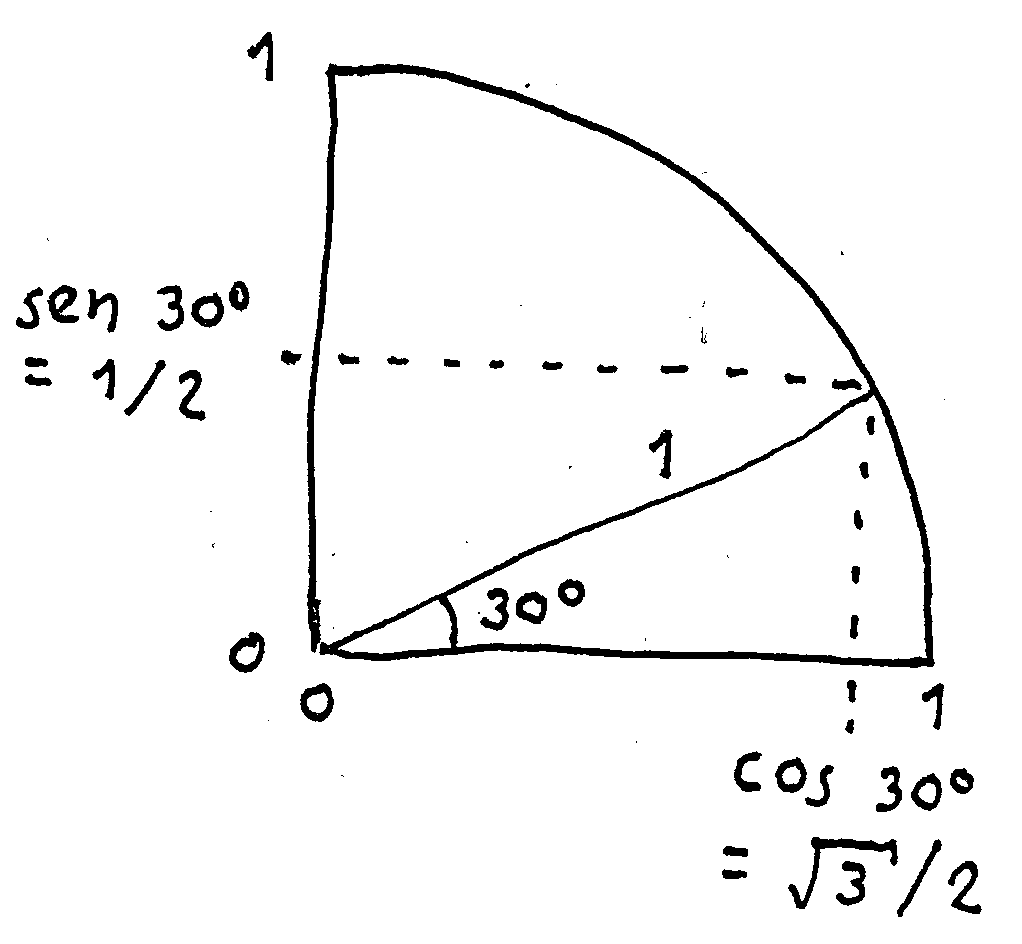
\includegraphics[height=3cm]{2021-1-C3/20210806_silvanus_triang_circ.pdf}
}
\quad
% (find-latexscan-links "C3" "20210806_silvanus_triang_1")
% (find-xpdf-page "~/LATEX/2021-1-C3/20210806_silvanus_triang_1.pdf")
\myvcenter{
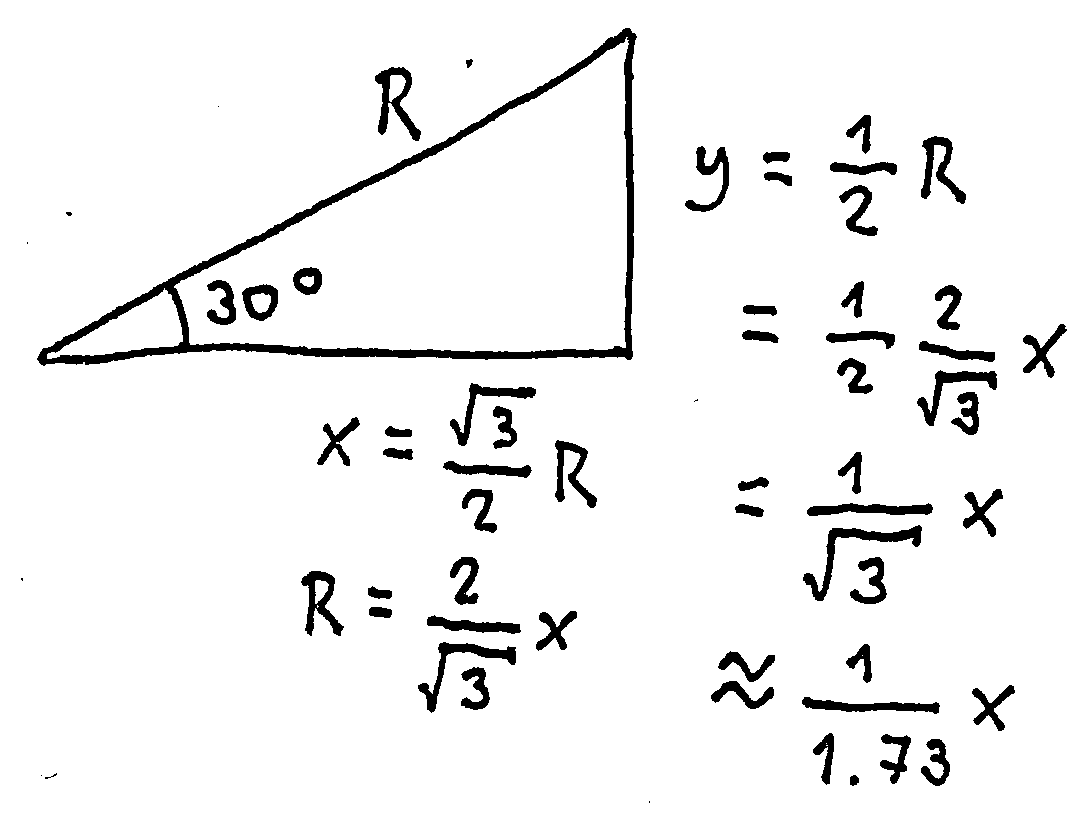
\includegraphics[height=3cm]{2021-1-C3/20210806_silvanus_triang_1.pdf}
}
\quad
% (find-latexscan-links "C3" "20210806_silvanus_triang_a_d")
% (find-xpdf-page "~/LATEX/2021-1-C3/20210806_silvanus_triang_a_d.pdf")
\myvcenter{
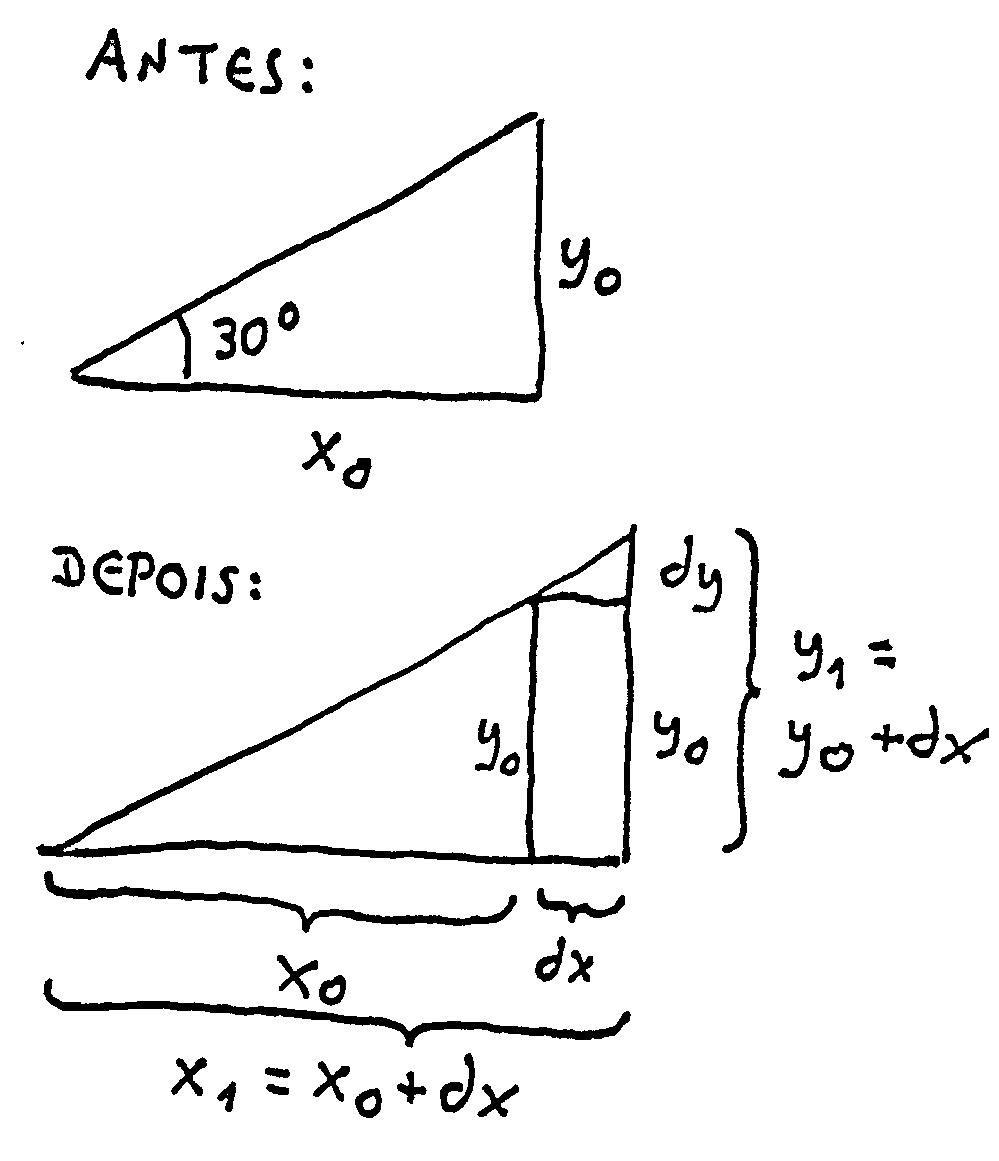
\includegraphics[height=4cm]{2021-1-C3/20210806_silvanus_triang_a_d.pdf}
}
$$

\newpage

{\bf Silvanus Thompson: o exemplo da escada (p.11)}


Links:

{\scriptsize

% (find-sthompsonpage (+ 11  11)   "ladder")
% (find-sthompsontext (+ 11  11)   "ladder")
% https://www.gutenberg.org/files/33283/33283-pdf.pdf#page=22
\url{https://www.gutenberg.org/files/33283/33283-pdf.pdf#page=22}

\url{http://angg.twu.net/eev-videos/2021-1-C3-notacao-de-fisicos-s-esc.mp4}

}

$$
% (find-latexscan-links "C3" "20210806_silvanus_escada_3d")
% (find-xpdf-page "~/LATEX/2021-1-C3/20210806_silvanus_escada_3d.pdf")
\myvcenter{
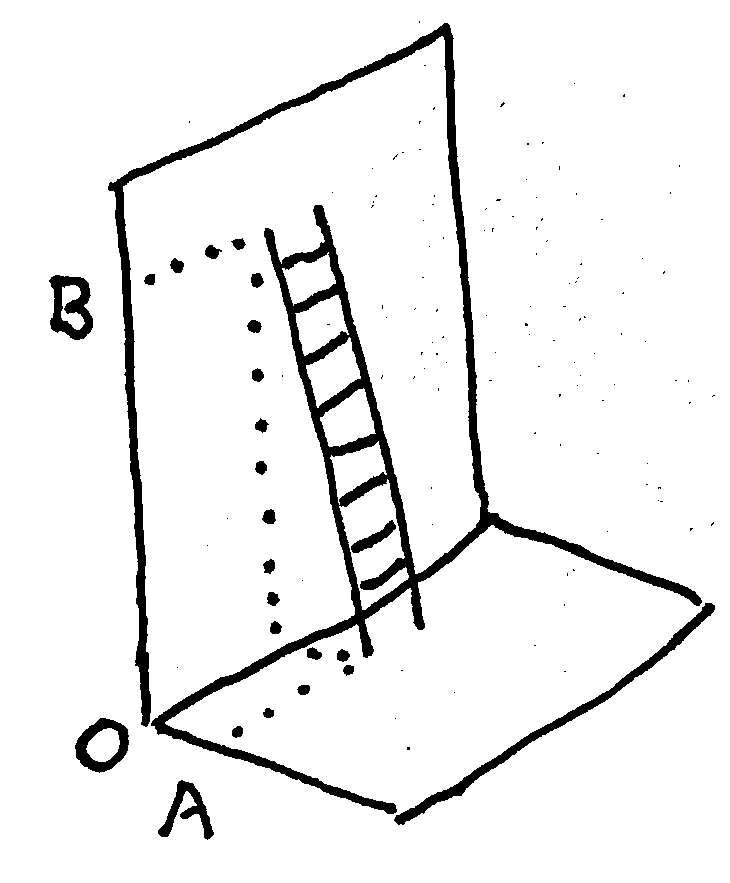
\includegraphics[height=3cm]{2021-1-C3/20210806_silvanus_escada_3d.pdf}
}
\quad
% (find-latexscan-links "C3" "20210806_silvanus_escada")
% (find-xpdf-page "~/LATEX/2021-1-C3/20210806_silvanus_escada.pdf")
\myvcenter{
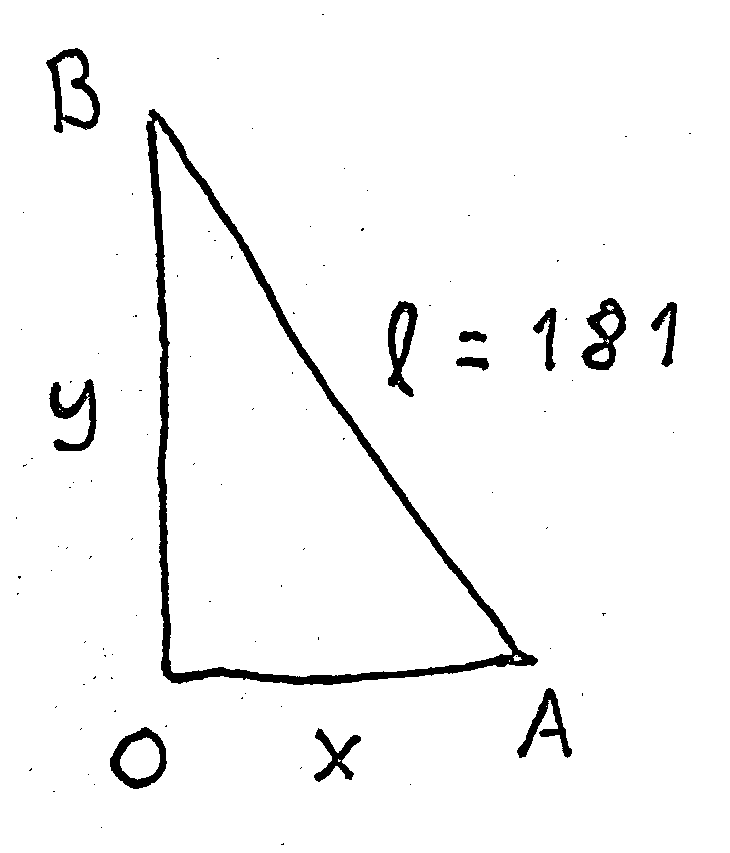
\includegraphics[height=3cm]{2021-1-C3/20210806_silvanus_escada.pdf}
}
\quad
% (find-latexscan-links "C3" "20210806_silvanus_escada_antes")
% (find-xpdf-page "~/LATEX/2021-1-C3/20210806_silvanus_escada_antes.pdf")
\myvcenter{
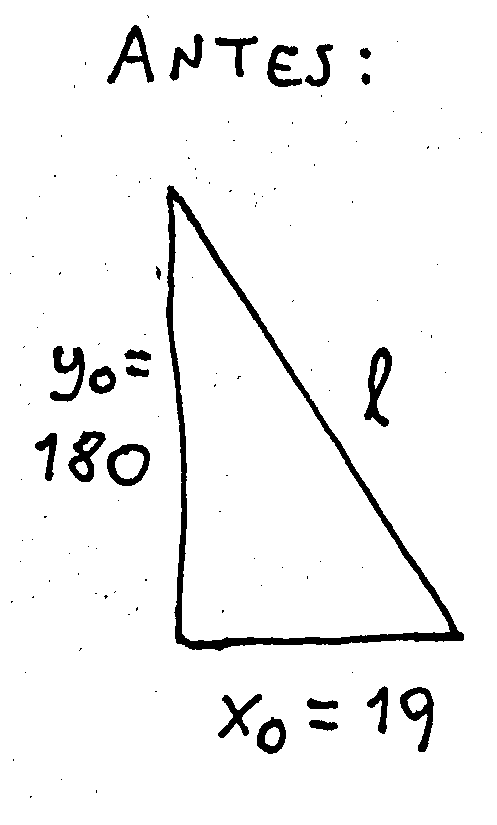
\includegraphics[height=3.2cm]{2021-1-C3/20210806_silvanus_escada_antes.pdf}
}
\quad
% (find-latexscan-links "C3" "20210806_silvanus_escada_depois")
% (find-xpdf-page "~/LATEX/2021-1-C3/20210806_silvanus_escada_depois.pdf")
\myvcenter{
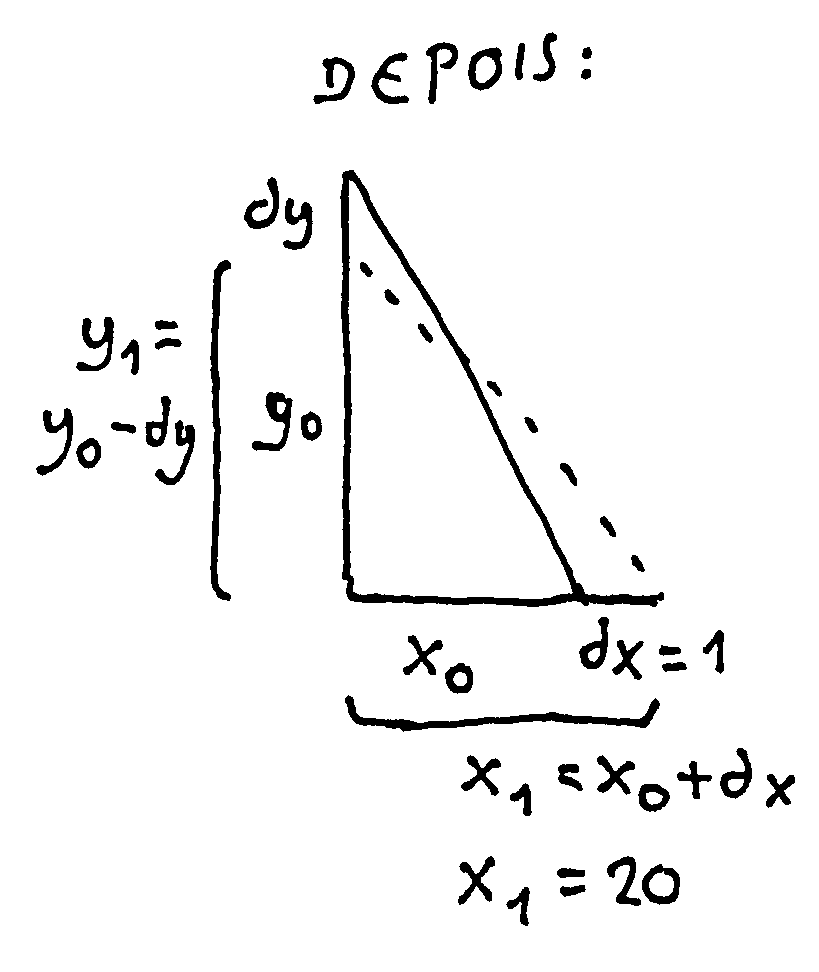
\includegraphics[height=4cm]{2021-1-C3/20210806_silvanus_escada_depois.pdf}
}
$$


\newpage

{\bf Silvanus Thompson: o exemplo da escada: contas}

\msk

% (find-latexscan-links "C3" "20210806_silvanus_escada_contas")
% (find-xpdf-page "~/LATEX/2021-1-C3/20210806_silvanus_escada_contas.pdf")
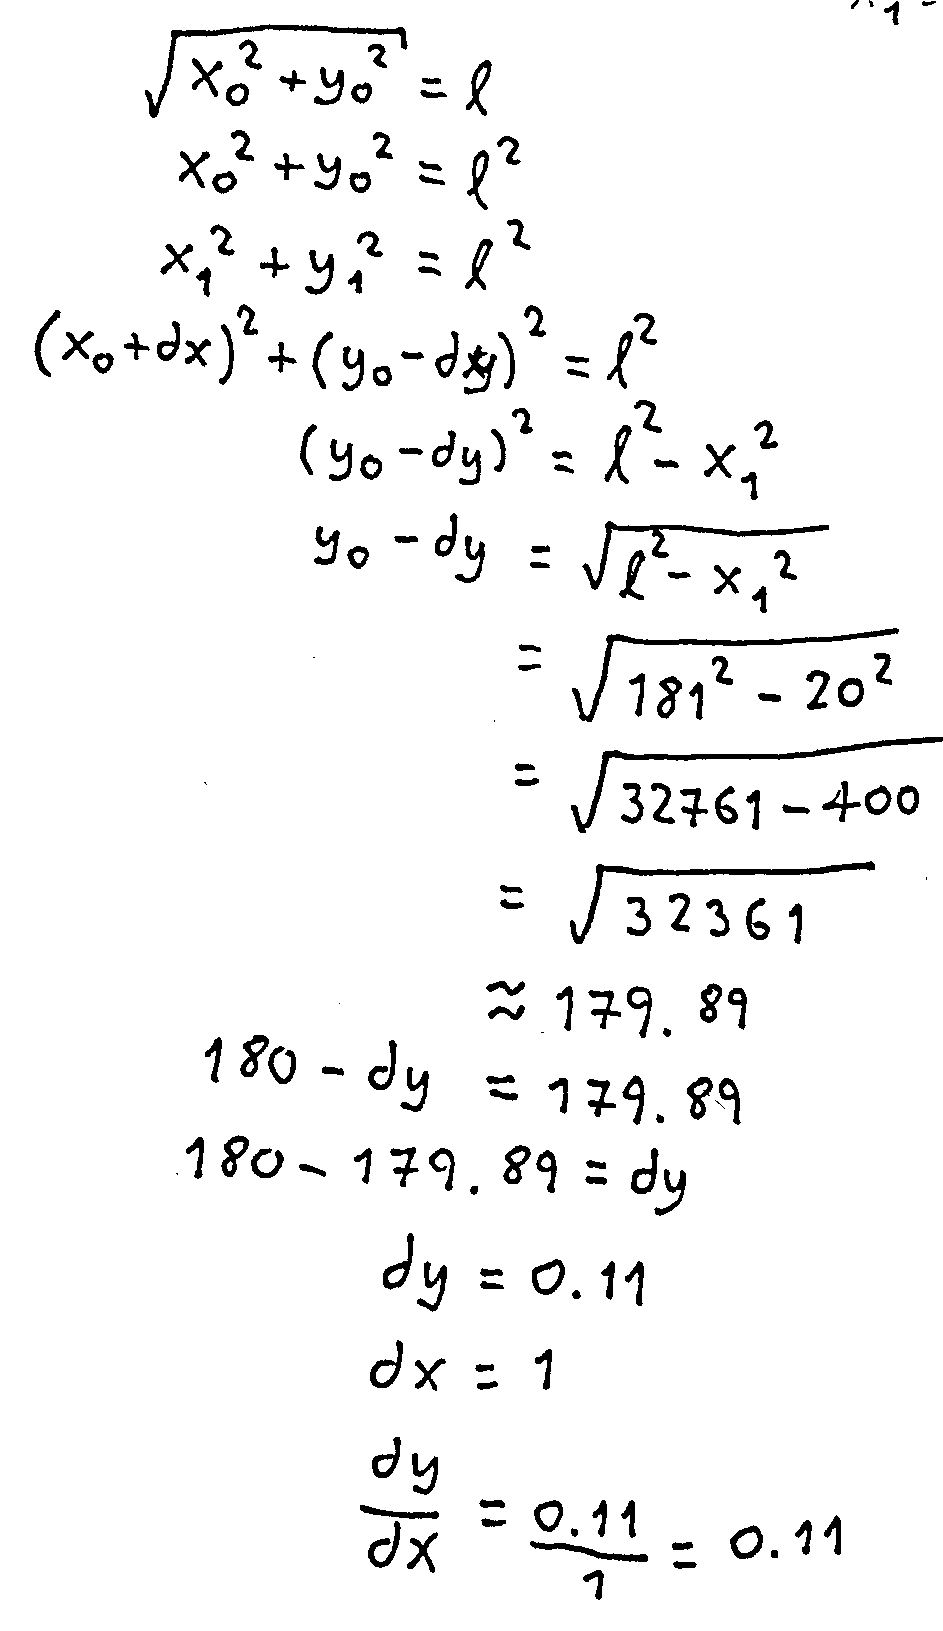
\includegraphics[height=7.0cm]{2021-1-C3/20210806_silvanus_escada_contas.pdf}

\newpage


Tudo que vem depois daqui vai ser reescrito.

\newpage

% «quadraticas-exemplos»  (to ".quadraticas-exemplos")
% (c3m211nfp 18 "quadraticas-exemplos")
% (c3m211nfa    "quadraticas-exemplos")
% (c3m211qp 2 "figuras-3D")
% (c3m211qa   "figuras-3D")

{\bf Quadratics - tests}


% (c3m211cnp 3 "exercicio-1")
% (c3m211cna   "exercicio-1")

% (find-LATEX "2021-1-C3-3D.lua" "QuadraticFunction-tests")
%L
%L V3.__index.p1 = V{2, -0.5}
%L V3.__index.p2 = V{1,  1.5}
%L V3.__index.p3 = V{0,  2}
%L
%L V3.__index.p1 = V{2,   -0.5}
%L V3.__index.p2 = V{0.5, 1.7}
%L V3.__index.p3 = V{0,   0.5}

%L qf = QuadraticFunction {x0=3, y0=2, a=2, Dx=0, Dy=0, Dxx=0, Dyy=0, Dxy=1}
%L srf = Surface.new(qf, 3, 2)
\pu

\def\QuadraticInPerspective#1{
   \beginpicture(0,-3)(10,6)
     \pictgray{\expr{v3():xygrid(4,3)          }}
     \expr          {v3():axeswithticks(4,3,3) }
     \expr          {#1:diagonals(8, "c")      }
     \expr          {#1:square   (8, "0")      }
     \pictgray{\expr{#1:square   (2, "p")      }}
     \expr          {#1:square   (8, "c")      }
   \end{picture}}

$$\unitlength=10pt
  \QuadraticInPerspective{srf}
$$


\newpage

%L qf = QuadraticFunction {x0=3, y0=2, a=2, Dx=0, Dy=0, Dxx=1, Dyy=1, Dxy=0}
%L srf = Surface.new(qf, 3, 2)
\pu

$$\unitlength=10pt
  \QuadraticInPerspective{srf}
$$


\newpage

%L qf = QuadraticFunction {x0=3, y0=2, a=2, Dx=0, Dy=0, Dxx=1, Dyy=-1, Dxy=0}
%L srf = Surface.new(qf, 3, 2)
\pu

$$\unitlength=10pt
  \QuadraticInPerspective{srf}
$$


\newpage

% (c3m202planotangp 27 "3D-fig")
% (c3m202planotanga    "3D-fig")

% (find-LATEX "edrxgac2.tex" "beginpicture")

%L rv = savevars(function (...)
%L      ex,ey,vx,vy, A0, A,B,C,D,E,F,E,G = ... end,
%L      ex,ey,vx,vy, A0, A,B,C,D,E,F,E,G)
%L
%L ex = v3(1,0,0)
%L ey = v3(0,1,0)
%L vx = v3(0,0,0.5)
%L vy = v3(0,0,1.5)
%L vz = v3(0,0,0.5)
%L A0 = v3(2,1,0); B0 = A0 + ex; C0 = A0 + ey; D0 = B0 + ey
%L A  = A0 + vz
%L B  = A + ex
%L C  = A + ey
%L D  = A + ex + ey
%L E  = B + vx
%L F  = E + ey
%L G  = C + vy
%L H  = G + ex
%L I  = H + vx
%L
%L V3.__index.p1 = V{2, -0.5}
%L V3.__index.p2 = V{1,  1.25}
%L V3.__index.p3 = V{0,  2}
%L
\pu

$\vcenter{\hbox{%
 \unitlength=20pt
 \beginpicture(0,-4)(8,8)
%P \pictgray{<v3():xygrid(3,3)>}
%P <v3():axeswithticks(3,3,3)>
%P \pictgray{\Line<A0><A> \Line<B0><B> \Line<C0><C> \Line<D0><D>}
%P \Line<A><B><D><C><A>
%P \Line<A><E><B> \Line<E><F><I><E>
%P \Line<A><G><C> \Line<G><H><I><G>
%P \Line<D><F>
 \pu
 \end{picture}%
 }}
$
%

%L rv()
\pu


\newpage

% «thomas»  (to ".thomas")
% (find-books "__analysis/__analysis.el" "thomas")
% (find-thomas11-1page (+  25  159) "3.2" "Differentiation rules")
% (find-thomas11-1page (+  26  171) "3.3" "The derivative as a rate of change")
% (find-thomas11-1page (+  28  183) "3.4" "Derivatives of trigonometric functions")
% (find-thomas11-1page (+  30  190) "3.5" "The chain rule and parametric equations")
% (find-thomas11-1page (+  32  205) "3.6" "Implicit differentiation")
% (find-thomas11-1page (+  34  213) "3.7 Related Rates")
% (find-thomas11-1page (+  35  221) "3.8 Linearization and Differentials")

% «bortolossi»  (to ".bortolossi")
% (find-bortolossi7page (+ -238 256)    "matriz jacobiana")
% (find-bortolossi7page (+ -238 261)    "Teorema 7.6")
% (find-bortolossi7page (+ -238 263) "7.3. Composição de funções")
% (find-bortolossi7page (+ -238 266) "7.5. A regra da cadeia em Cálculo 2")
% (find-bortolossi7page (+ -238 266)    "Teorema 7.7")

% «segundo-exemplo»  (to ".segundo-exemplo")
% (c3m211nfp 6 "segundo-exemplo")
% (c3m211nfa   "segundo-exemplo")

{\bf Um segundo exemplo}

Digamos que o conjunto dos pontos $(x,y)$

``que obedecem as restrições'' é esse aqui:
%
$$\setofst{(x,y)∈\R^2}{x^2+y^2=5}$$

e que $(x_0,y_0) = (3,4)$.

\bsk
\bsk

Os físicos consideram que ``é óbvio'' que (em geral!) variáveis

``variam continuamente'', então se $x_1=x_0+Δx$ e $y_1=y_0+Δy$

e $Δx$ é muito pequeno então $Δy$ é muito pequeno também.

(Veja o vídeo!...)


\newpage

{\bf O contexto importa muito}


\newpage

{\bf Exercício 1 (versão preliminar)}

Digamos que:

$$\begin{array}{rcl}
  \end{array}
$$



% z = x + y
% y = x


% O meu modo preferido de formalizar a notação de físicos é esse aqui.

% Silvanus P. Thompson:
% (find-books "__analysis/__analysis.el" "silvanus")
% (find-books "__analysis/__analysis.el" "kelley" "complete_idiots_guide")
% https://calculusmadeeasy.org/2.html negligible
% https://calculusmadeeasy.org/16.html


%\printbibliography

\GenericWarning{Success:}{Success!!!}  % Used by `M-x cv'

\end{document}

%  ____  _             _         
% |  _ \(_)_   ___   _(_)_______ 
% | | | | \ \ / / | | | |_  / _ \
% | |_| | |\ V /| |_| | |/ /  __/
% |____// | \_/  \__,_|_/___\___|
%     |__/                       
%
% «djvuize»  (to ".djvuize")
% (find-LATEXgrep "grep --color -nH --null -e djvuize 2020-1*.tex")

 (eepitch-shell)
 (eepitch-kill)
 (eepitch-shell)
# (find-fline "~/2021.1-C3/")
# (find-fline "~/LATEX/2021-1-C3/")
# (find-fline "~/bin/djvuize")

cd /tmp/
for i in *.jpg; do echo f $(basename $i .jpg); done

f () { rm -fv $1.png $1.pdf; djvuize $1.pdf }
f () { rm -fv $1.png $1.pdf; djvuize WHITEBOARDOPTS="-m 1.0"       $1.pdf; xpdf $1.pdf }
f () { rm -fv $1.png $1.pdf; djvuize WHITEBOARDOPTS="-m 1.0 -f 30" $1.pdf; xpdf $1.pdf }
f () { rm -fv $1.png $1.pdf; djvuize WHITEBOARDOPTS="-m 1.0 -f 45" $1.pdf; xpdf $1.pdf }
f () { rm -fv $1.png $1.pdf; djvuize WHITEBOARDOPTS="-m 0.5"       $1.pdf; xpdf $1.pdf }
f () { rm -fv $1.png $1.pdf; djvuize WHITEBOARDOPTS="-m 0.25"      $1.pdf; xpdf $1.pdf }
f () { cp -fv $1.png $1.pdf       ~/2021.1-C3/
       cp -fv        $1.pdf ~/LATEX/2021-1-C3/
       cat <<%%%
% (find-latexscan-links "C3" "$1")
%%%
}

f 20210806_silvanus_triang_1
f 20210806_silvanus_triang_a_d
f 20210806_silvanus_triang_circ

f 20210806_silvanus_escada
f 20210806_silvanus_escada_3d
f 20210806_silvanus_escada_antes
f 20210806_silvanus_escada_contas
f 20210806_silvanus_escada_depois

f 20210804_sqrt



%  __  __       _        
% |  \/  | __ _| | _____ 
% | |\/| |/ _` | |/ / _ \
% | |  | | (_| |   <  __/
% |_|  |_|\__,_|_|\_\___|
%                        
% <make>

 (eepitch-shell)
 (eepitch-kill)
 (eepitch-shell)
# (find-LATEXfile "2019planar-has-1.mk")
make -f 2019.mk STEM=2021-1-C3-notacao-de-fisicos veryclean
make -f 2019.mk STEM=2021-1-C3-notacao-de-fisicos pdf

% Local Variables:
% coding: utf-8-unix
% ee-tla: "c3nf"
% ee-tla: "c3m211nf"
% End:
